\section{Adversarial tree search}

Consider a deterministic zero-sum two-player game as a 4-tuple 
$G = (S, A, T, U)$, where $S$ is the set of all states, $A$ is the
set of all actions, some of which may not be applicable in some
states and $T: S \times A \rightarrow S$ is the transition function
describing the result of taking a certain action in a certain state.
Let $S^\circ \subset S$ be the set of all terminal states, 
then $U: S^\circ \rightarrow \mathrm{R}$ is the utility function 
associating each terminal state with a real number. Since not all
actions are applicable in all states, let $A(s) \subseteq A$ denote
the subset of actions that are applicable in the state $s$.

To enforce the zero-sum property, the first player to take action will
recieve a utility of $U(s)$ in terminal states, while the second player
recieves $-U(s)$. The first player will be reffered to as the Max player,
and the second as the Min player, as they seek to respectively maximize 
and minimize the utility function.

The question is now, given a state $s_0 \in S$, what action should
a rational agent take? To answer this question, we model the game
as a game tree, starting with a root node containing the current state
$s_0$. Each node $n$ in the game tree has a set of children
$n.children = \{ T(n.state, a) \; | \; a \in A(n.state) \}$, that
is exactly one node for each state reachable from $n.state$ by 
an applicable action.

\begin{figure}[H]
    \centering

    \tikzset{
    max node/.style={circle,draw,inner sep=5},
    min node/.style={circle,draw,inner sep=5, fill=gray}
    }

    \begin{tikzpicture}[scale=12]
    % Specify spacing for each level of the tree
    \tikzstyle{level 1}=[level distance=1.7mm,sibling distance=4mm]
    \tikzstyle{level 2}=[level distance=1.7mm,sibling distance=2mm]
    % The Tree
    \node(0)[max node]{$s_0$}
    child{node(1)[min node]{$s_1$}
        child{node[max node, label=below:{$U(s_3)=1$}]{$s_3$}
            edge from parent node[left]{$a_0$}
        }
        child{node[max node, label=below:{$U(s_4)=-1$}]{$s_4$}
            edge from parent node[right]{$a_1$}
        }
        edge from parent node[left]{$a_0$}
    }
    child{node(2)[min node]{$s_2$}
        child{node[max node]{$s_5$}
            child{node[min node, label=below:{$U(s_6)=0$}]{$s_6$}
                edge from parent node[left]{$a_0$}
            }
            child{node[min node, label=below:{$U(s_4)=-1$}]{$s_4$}
                edge from parent node[right]{$a_1$}
            } 
            edge from parent node[right]{$a_0$}
        }
        edge from parent node[right]{$a_1$}
    };

    \end{tikzpicture}

    \caption{A simple game tree where white nodes correspond to the
    Max player's turn, and grey nodes to the Min player's. Notice how
    not all actions are applicable in all states, terminal states do
    not have to be on the same depth, and a given terminal state will have
    the same utility regardless of the path leading to it.}
    \label{fig:game_tree}

\end{figure}


In the game from figure \ref{fig:game_tree}, it is easy to see that in
order to maximize the utility function, the Max player should take action
$a_1$, forcing the Min player into action $a_0$, and then taking $a_0$
for a utility of $0$. While a higher utility is available in the subtree
stemming from first taking $a_0$, an optimal Min player would pick $a_1$
every time, leading to a worse outcome for Max.

While it is easy to see these optimal decisions in a small game tree, even
Tic Tac Toe has a game tree complexity (the number of nodes in the game 
tree) on the order of $10^5$, while games like Chess and Go reach 
$10^{123}$ and $10^{360}$ respectively. Trees of these sizes are currently
impossible to search completely, so in order to construct a game playing
agent based on tree search methods, it is necessary to reduce the amount
of nodes that needs to be searched.

\subsection{MiniMax}

The classical approach to adversarial search, minimax builds on the
idea of minimizing the maximum amount of utility that your opponent can
achieve, in other words making their optimal choice as bad as possible.
The minimax value of a state can be recursively defined as

\begin{equation}
    MiniMax(s) = \begin{cases}
        U(s) & s \in S^\circ \\
        \max_{a \in A(s)} MiniMax(R(s, a)) & Player(s) = Max \\
        \min_{a \in A(s)} MiniMax(R(s, a)) & Player(s) = Min
    \end{cases}
    \label{eq:minimax}
\end{equation}
where $Player(s)$ returns the player which turn it is to take action in
state $s$. From this optimal play can be achieved by following the policy
given by:
\begin{equation}
    TakeAction(s) = \begin{cases}
        \arg\max_{a \in A(s)} MiniMax(R(s, a)) & Player(s) = Max \\
        \arg\min_{a \in A(s)} MiniMax(R(s, a)) & Player(s) = Min
    \end{cases}
    \label{eq:minimax_policy}
\end{equation}
This means that optimal play for the Max player simply consists of choosing
the action which leads to the state with the highest minimax value, and
vice versa for the Min player. The pseudocode for implementing minimax
is as follows:

\begin{algorithm}[H]
    \caption{Pure MiniMax search}
    \label{alg:minimax}
    \begin{algorithmic}[1]
    
    \Procedure{MiniMax}{$s$}
        \State \Return $\arg\max_{a \in A(s)} \textproc{MinValue}(R(s, a))$
    \EndProcedure
    \end{algorithmic}

    \begin{algorithmic}[1]

    \Procedure{MaxValue}{$s$}
        \If{$s \in S^\circ$}
            \Return $U(s)$
        \EndIf
        \State $v \leftarrow -\infty$
        \For{$a \in A(s)$}
            \State $v \leftarrow \max(v, \textproc{MinValue}(R(s, a)))$
        \EndFor
        \State \Return $v$
    \EndProcedure
    
    \end{algorithmic}
        
    \begin{algorithmic}[1]

    \Procedure{MinValue}{$s$}
        \If{$s \in S^\circ$}
            \Return $U(s)$
        \EndIf
        \State $v \leftarrow \infty$
        \For{$a \in A(s)$}
            \State $v \leftarrow \min(v, \textproc{MaxValue}(R(s, a)))$
        \EndFor
        \State \Return $v$
    \EndProcedure

    \end{algorithmic}
\end{algorithm}

Since minimax is essentially a depth first
search (DFS) with added backup of the minimax values, it has a time complexity
of $\mathcal{O}(b^m)$ and a space complexity of $\mathcal{O}(m)$,
where $b$ is the average number of applicable actions, also called the 
branching factor, and $m$ is the depth of the deepest node in the game tree.
Most notably however, is that it searches the \textit{entire}
game tree, making it infeasible for the vast majority of games.

Two main methods exist to make minimax practical on large 
game trees: depth limited search, and $\alpha\beta$-pruning.
These methods are compatible, and most if not all modern methods
implement both. 

The simplest of the two methods is depth limited search, which
as the name suggests terminates the recursion at a predetermined
depth instead of continuing to a terminal state. However, from 
the definition of games in the beginning of this section it is
clear that only terminal states have a utility value, so the
algorithm has nothing to return if recursion stops earlier. To
overcome this issue, an evaluation function 
$E: S \rightarrow \mathbb{R}$ is introduced, representing an
estimate of the true minimax value of the position \revise. 
This evaluation function can be based on domain knowledge e.g.
piece values and positioning principles in chess, it can be
learned using neural networks, or it can be a combination of both.
Since the algorithm no longer searches the entire game tree and
uses an approximation for the minimax value, it is no longer
guaranteed optimal, but can still produce strong play with a good
evaluation function.

$\alpha\beta$-pruning can be thought of as a simplification of
the minimax formula that is applicable in certain cases, and
as such it still guarantees optimality. Consider the following
example:
\begin{align*}
    Minimax(s) &= \max(MiniMax(R(s, a_0)), MiniMax(R(s, a_1)), 
    MiniMax(R(s, a_2))) \\
    &= \max(\min(5, 12, 8), \min(x_0, 1, x_1), \min(12, x_2, 4)) \\
    &= \max(5, y_0, y_1), \;\; y_0 \leq 1, \; y_1 \leq 4 \\
    &= 5
\end{align*}
On the second line some values are missing, but the values that are present
can be used to set an upper bound for their corresponding $\min$ statements,
which in turn can be used to determine the value of the $\max$ statement.
This method can be used all throughout the minimax algorithm, potentially
cutting off huge subtrees from the search space, allowing it to search much
deeper. Since the example is very shallow, it does not illustrate this 
to full effect, but if the actions are expanded in the optimal order, 
$\alpha\beta$-pruning has a time complexity of $\mathcal{O}(b^{m/2})$, which
compared to minimax's $\mathcal{O}(b^{m})$ lets $\alpha\beta$-pruning search
twice as deep in the same time. In practice the actions cannot be expanded
in the optimal order since an optimal ordering could be used to play the
game optimally, but existing methods can get quite close to the theoretical
limit \needcit.

\begin{algorithm}[H]
    \caption{Depth Limited Minimax with $\alpha\beta$-Pruning}
    \label{alg:alphabeta}
    \begin{algorithmic}[1]
    
    \Procedure{Alpha-Beta}{$s$, $d$}
        \State \Return $\arg\max_{a \in A(s)}$ Min-Value(R(s, a))
    \EndProcedure
    \end{algorithmic}

    \begin{algorithmic}[1]

    \Procedure{MaxValue}{$s$, $\alpha$, $\beta$, $d$}
        \If{$s \in S^\circ$ \textbf{or} $d=0$}
            \Return $E(s)$
        \EndIf
        \State $v \leftarrow -\infty$
        \For{$a \in A(s)$}
            \State $v \leftarrow \max(v, MinValue(R(s, a), \alpha, \beta, d-1))$
            \If{$v \geq \beta$}
                \Return $v$
            \EndIf
            \State $\alpha \leftarrow \max(\alpha, v)$
        \EndFor
        \State \Return $v$
    \EndProcedure
    
    \end{algorithmic}
        
    \begin{algorithmic}[1]

    \Procedure{MinValue}{$s$, $\alpha$, $\beta$, $d$}
        \If{$s \in S^\circ$ \textbf{or} $d=0$}
            \Return $E(s)$
        \EndIf
        \State $v \leftarrow \infty$
        \For{$a \in A(s)$}
            \State $v \leftarrow \min(v, MaxValue(R(s, a), \alpha, \beta, d-1))$
            \If{$v \leq \alpha$}
                \Return $v$
            \EndIf
            \State $\beta \leftarrow \min(\beta, v)$
        \EndFor

        \State \Return $v$
    \EndProcedure

    \end{algorithmic}
\end{algorithm}

\subsection{Monte Carlo Tree Search}

Monte Carlo methods in AI rely on information from many simulated games 
played with randomly selected actions to guide decision making in the 
current state. In its most basic form, Monte Carlo sampling generates
all successors $\{ Result(s, a) \;|\; a \in A(s) \}$ of the current
state, and simulates multiple games starting from each successor state
until the budget runs out. These simulated games are called rollouts,
and the budget can either be a fixed number of rollouts, or a time
limit. When the budget runs out, the action leading to the successor
state with the highest average utility is chosen as the next action.

\begin{figure}[H]
    \centering
    
    \tikzset{
    state/.style={circle,draw,inner sep=5},
    win/.style={circle,draw,inner sep=2},
    loss/.style={circle,draw,inner sep=2, fill=black}
    }
    
    \begin{tikzpicture}[scale=12]
    % Specify spacing for each level of the tree
    \tikzstyle{level 1}=[level distance=1.7mm,sibling distance=2.5mm]
    \tikzstyle{level 2}=[level distance=2.5mm,sibling distance=.3mm]
    % The Tree
    \node(0)[state]{$s_0$}
    child{node[state, label=left:{\small $\hat{U}=0.25$}]{$s_1$}
    child{node[win]{}
        edge from parent[decorate, decoration=snake] node[left]{Rollouts}
        }
        child{node[loss]{}
        edge from parent[decorate, decoration=snake]
        }
        child{node[loss]{}
        edge from parent[decorate, decoration=snake]
        }
        child{node[loss]{}
        edge from parent[decorate, decoration=snake]
        }
        edge from parent node[right]{$a_0$}
    }
    child{node[state, label=left:{\small $\hat{U}=0.75$}]{$s_2$}
        child{node[win]{}
        edge from parent[decorate, decoration=snake]
        }
        child{node[loss]{}
        edge from parent[decorate, decoration=snake]
        }
        child{node[win]{}
        edge from parent[decorate, decoration=snake]
        }
        child{node[win]{}
        edge from parent[decorate, decoration=snake]
        }
        edge from parent node[right]{$a_1$}
    }
    child{node[state, label=left:{\small $\hat{U}=0.5$}]{$s_3$}
        child{node[win]{}
        edge from parent[decorate, decoration=snake]
        }
        child{node[loss]{}
        edge from parent[decorate, decoration=snake]
        }
        child{node[win]{}
        edge from parent[decorate, decoration=snake]
        }
        child{node[loss]{}
        edge from parent[decorate, decoration=snake]
        }
        edge from parent node[right]{$a_2$}
    };

    \end{tikzpicture}

    \caption{The simplest Monte Carlo method, with a budget of 12 total
    rollouts. White leaf nodes
    corresponds to wins, and black to losses. Action $a_1$ maximizes
    the average utility $\hat{U}$ at 0.75, and is therefore the move chosen.}
    \label{fig:simple_monte_carlo}

\end{figure}

Monte Carlo Tree Search (MCTS) expands the classical idea of Monte Carlo
sampling by expanding a partial game tree containing the results of
the simulations, and using these results to guide further simulations.
Nodes in the game tree store the following information:

\begin{lstlisting}
class MCTSTreeNode:
    State: GameState
    Count: Number
    Utility: Number
    Children: MCTSTreeNode[]
    UnexpandedActions: GameAction[]
\end{lstlisting}

At creation, each nodes \lstinline|UnexpandedActions| list is initialized
with the applicable actions from its \lstinline|State|. To build up the 
game tree, a root \lstinline|MCTSTreeNode| is created containing the 
current game state, and then each iteration of the algorithm goes through 
the following steps:

\begin{enumerate}
    \item Select
    \item Expand
    \item Simulate
    \item Backpropagate
\end{enumerate}

\textbf{Select:} The selection step starts in the root of the tree,
and progresses recursively down through the tree using the following
rules: If the node contains a terminal state, or the node still has
unexpanded actions, return the node. Otherwise, run the selection
step again on the child with the highest $UCB1$ value:

\begin{equation}
    \text{UCB1}(Node) = \frac{Utility}{Count} + 
    c\sqrt{\frac{\log{Parent.Count}}{Count}}
\end{equation}

The first term in UCB1 is called the exploitation term, and represents
an estimate of the utility of the node. This makes sure that the algorithm
gravitates toward states with a high utility. The second term is the
exploration term, which increases the value of nodes that have not been
picked much compared to their parents. This prevents the algorithm from
getting stuck on suboptimal nodes in case the initial few rollouts from
the parent are a bad estimation of their true utility. The application
of UCB1 on trees is usually called UCT, or Upper Confidence bounds on Trees.

\textbf{Expand:} In the expansion step, the selected node is expanded by 
popping an action from \lstinline|UnexpandedActions|, and adding a child 
node containing the successor state corresponding to that action. This
child node is then also returned. If the selected node contains a terminal 
state or has no unexpanded actions, the selected node is returned instead.

\textbf{Simulate:} Starting from the state in the expanded node, a rollout
is performed. As previously noted, a rollout consists of taking random
actions until a terminal state is reached, and then returning the utility
of that state.

\textbf{Backpropagate:} Starting at the expanded node, \lstinline|Count| is 
incremented by $1$. If it is the Max players turn to move in 
\lstinline|State|, \lstinline|Utility| is incremented by the utility
returned in the simulation step, otherwise it is incremented by $1$ minus
that utility. This is to keep the UCT algorithm from having to switch
signs for the different players.

\begin{figure}[H]
    \centering

    \tikzset{
    max/.style={circle,draw,inner sep=5},
    min/.style={circle,draw,inner sep=5, fill=gray},
    bold/.style={line width=1mm},
    thin/.style={line width=0.2mm}
    }

    % Specify spacing for each level of the tree
    \tikzstyle{level 1}=[level distance=1.7mm,sibling distance=4mm]
    \tikzstyle{level 2}=[level distance=1.7mm,sibling distance=2mm]
    
    \begin{tabular}{cc}
        
    \begin{subfigure}[b]{0.4\textwidth}
        \centering
        \resizebox{\textwidth}{!}{
            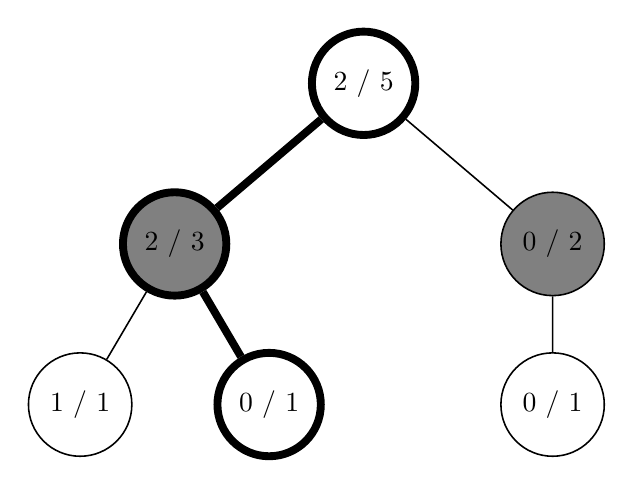
\begin{tikzpicture}[bold, scale=12]
                % The Tree
                \node(0)[max]{2 / 5}
                child{node[min]{2 / 3}
                    child{node[max, thin]{1 / 1} edge from parent[thin]}
                    child{node[max]{0 / 1}}
                }
                child{[thin]node[min]{0 / 2}
                    child{node[max]{0 / 1}}
                };
            \end{tikzpicture}
        }
        \caption*{Selection}
    \end{subfigure}
    &
    \begin{subfigure}[b]{0.4\textwidth}
        \centering
        \resizebox{\textwidth}{!}{
            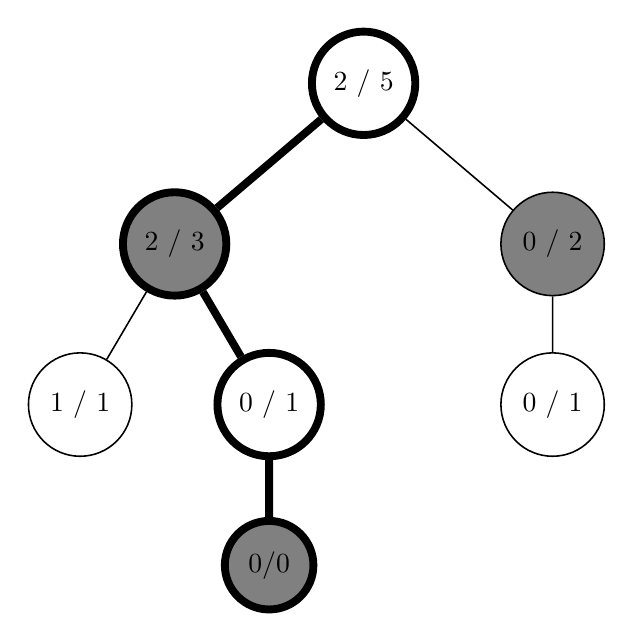
\begin{tikzpicture}[bold, scale=12]
                % The Tree
                \node(0)[max]{2 / 5}
                child{node[min]{2 / 3}
                    child{node[max, thin]{1 / 1} edge from parent[thin]}
                    child{node[max]{0 / 1}
                        child{node[min]{0/0}}
                    }
                }
                child{[thin]node[min]{0 / 2}
                    child{node[max]{0 / 1}}
                };
            \end{tikzpicture}
        }
        \caption*{Expansion}
    \end{subfigure}
    \\
    \begin{subfigure}[b]{0.4\textwidth}
        \centering
        \resizebox{\textwidth}{!}{
            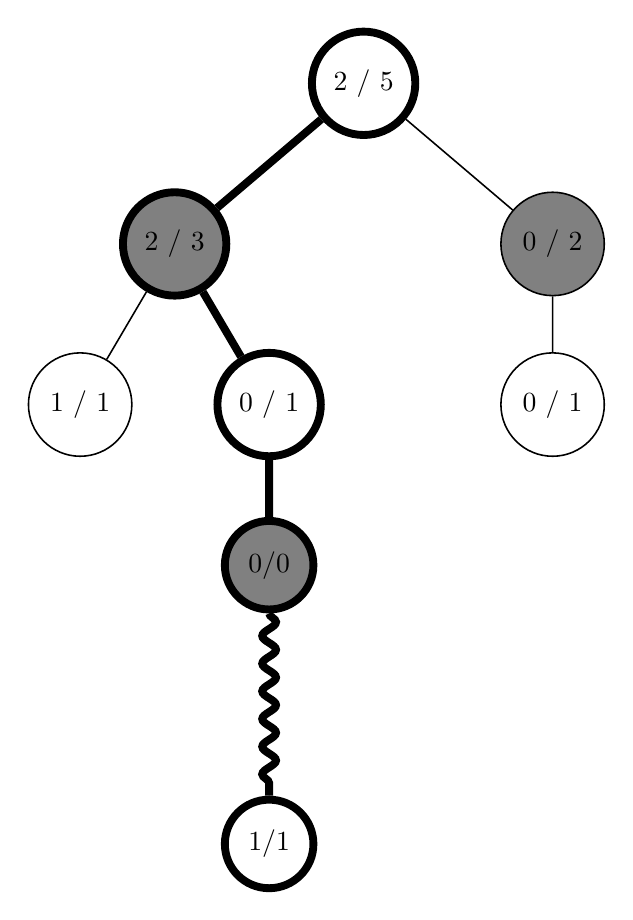
\begin{tikzpicture}[bold, scale=12]
                % The Tree
                \node(0)[max]{2 / 5}
                child{node[min]{2 / 3}
                    child{node[max, thin]{1 / 1} edge from parent[thin]}
                    child{node[max]{0 / 1}
                        child{node[min]{0/0}
                            child{node[max, yshift=-1.5cm]{1/1} edge from parent[decorate, decoration=snake]}
                        }
                    }                }
                child{[thin]node[min]{0 / 2}
                    child{node[max]{0 / 1}}
                };
            \end{tikzpicture}
        }
        \caption*{Simulation}
    \end{subfigure}
    &
    \begin{subfigure}[b]{0.4\textwidth}
        \centering
        \resizebox{\textwidth}{!}{
            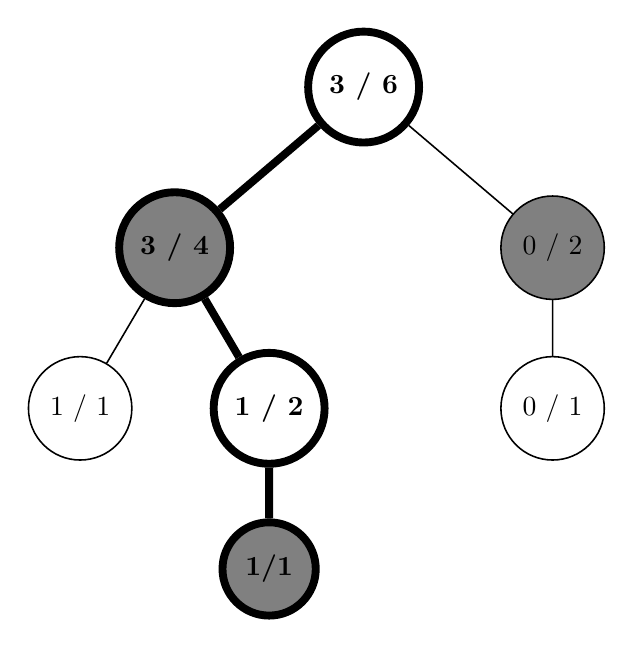
\begin{tikzpicture}[bold, scale=12]
                % The Tree
                \node(0)[max]{\textbf{3 / 6}}
                child{node[min]{\textbf{3 / 4}}
                    child{node[max, thin]{1 / 1} edge from parent[thin]}
                    child{node[max]{\textbf{1 / 2}}
                        child{node[min]{\textbf{1/1}}}
                    }
                }
                child{[thin]node[min]{0 / 2}
                    child{node[max]{0 / 1}}
                };
            \end{tikzpicture}
        }
        \caption*{Backpropagation}
    \end{subfigure}

    \end{tabular}


   
    \caption{One iteration of MCTS on an example graph. Node labels signify utility / count. Note that the count of each non-root node is equal to the sum of the count of its children plus one, since a simulation was also performed when the node was originally expanded. Likewise the utility can be one higher than the sum of child utilities if the simulation was a Max player win.}
    \label{fig:mcts_illustrated}

\end{figure}


An implementation of the MCTS algorithm can look like this:

\begin{figure}[H]
    \centering

    \tikzset{
    max/.style={circle,draw,inner sep=5},
    min/.style={circle,draw,inner sep=5, fill=gray},
    bold/.style={line width=1mm},
    thin/.style={line width=0.2mm}
    }

    % Specify spacing for each level of the tree
    \tikzstyle{level 1}=[level distance=1.7mm,sibling distance=4mm]
    \tikzstyle{level 2}=[level distance=1.7mm,sibling distance=2mm]
    
    \begin{tabular}{cc}
        
    \begin{subfigure}[b]{0.4\textwidth}
        \centering
        \resizebox{\textwidth}{!}{
            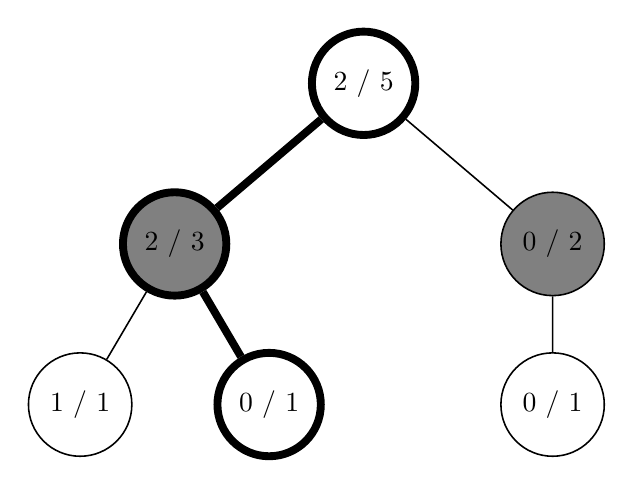
\begin{tikzpicture}[bold, scale=12]
                % The Tree
                \node(0)[max]{2 / 5}
                child{node[min]{2 / 3}
                    child{node[max, thin]{1 / 1} edge from parent[thin]}
                    child{node[max]{0 / 1}}
                }
                child{[thin]node[min]{0 / 2}
                    child{node[max]{0 / 1}}
                };
            \end{tikzpicture}
        }
        \caption*{Selection}
    \end{subfigure}
    &
    \begin{subfigure}[b]{0.4\textwidth}
        \centering
        \resizebox{\textwidth}{!}{
            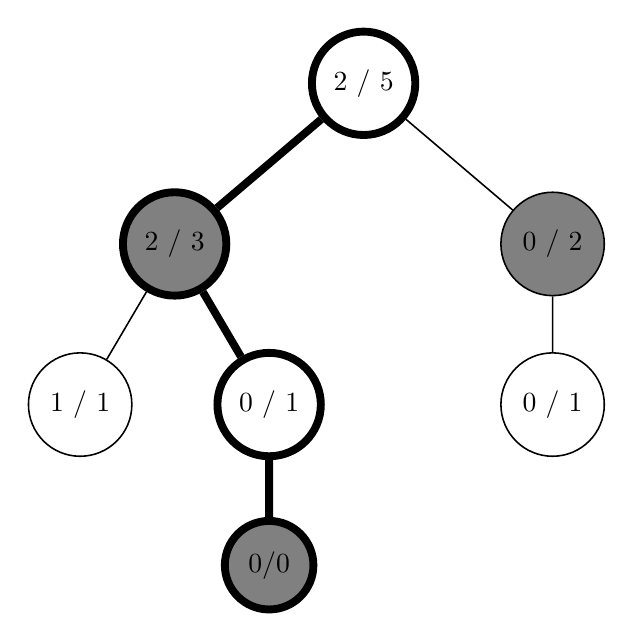
\begin{tikzpicture}[bold, scale=12]
                % The Tree
                \node(0)[max]{2 / 5}
                child{node[min]{2 / 3}
                    child{node[max, thin]{1 / 1} edge from parent[thin]}
                    child{node[max]{0 / 1}
                        child{node[min]{0/0}}
                    }
                }
                child{[thin]node[min]{0 / 2}
                    child{node[max]{0 / 1}}
                };
            \end{tikzpicture}
        }
        \caption*{Expansion}
    \end{subfigure}
    \\
    \begin{subfigure}[b]{0.4\textwidth}
        \centering
        \resizebox{\textwidth}{!}{
            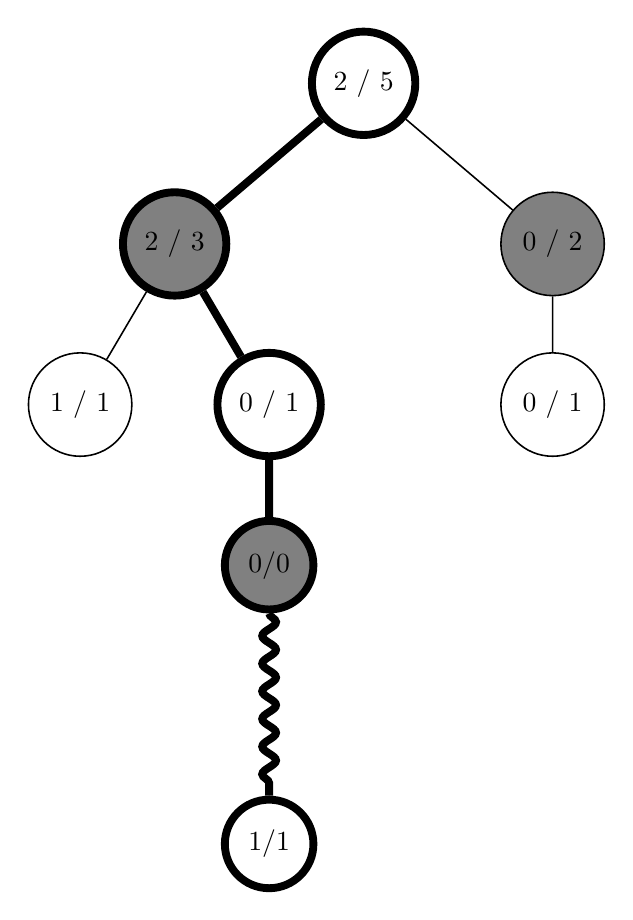
\begin{tikzpicture}[bold, scale=12]
                % The Tree
                \node(0)[max]{2 / 5}
                child{node[min]{2 / 3}
                    child{node[max, thin]{1 / 1} edge from parent[thin]}
                    child{node[max]{0 / 1}
                        child{node[min]{0/0}
                            child{node[max, yshift=-1.5cm]{1/1} edge from parent[decorate, decoration=snake]}
                        }
                    }                }
                child{[thin]node[min]{0 / 2}
                    child{node[max]{0 / 1}}
                };
            \end{tikzpicture}
        }
        \caption*{Simulation}
    \end{subfigure}
    &
    \begin{subfigure}[b]{0.4\textwidth}
        \centering
        \resizebox{\textwidth}{!}{
            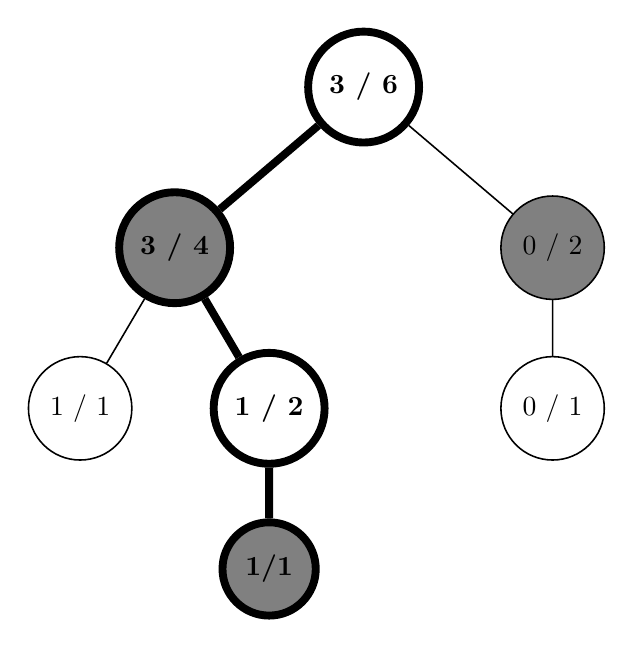
\begin{tikzpicture}[bold, scale=12]
                % The Tree
                \node(0)[max]{\textbf{3 / 6}}
                child{node[min]{\textbf{3 / 4}}
                    child{node[max, thin]{1 / 1} edge from parent[thin]}
                    child{node[max]{\textbf{1 / 2}}
                        child{node[min]{\textbf{1/1}}}
                    }
                }
                child{[thin]node[min]{0 / 2}
                    child{node[max]{0 / 1}}
                };
            \end{tikzpicture}
        }
        \caption*{Backpropagation}
    \end{subfigure}

    \end{tabular}


   
    \caption{One iteration of MCTS on an example graph. Node labels signify utility / count. Note that the count of each non-root node is equal to the sum of the count of its children plus one, since a simulation was also performed when the node was originally expanded. Likewise the utility can be one higher than the sum of child utilities if the simulation was a Max player win.}
    \label{fig:mcts_illustrated}

\end{figure}
